\documentclass[a4paper,11pt]{jsarticle}


% 数式
\usepackage{amsmath,amsfonts,amssymb}
\usepackage{bm}
% 画像
\usepackage[dvipdfmx]{graphicx}
\usepackage{siunitx}
\usepackage{wrapfig}
\usepackage{cases}
\usepackage{dcolumn}
\makeatletter
\newcommand{\figcaption}[1]{\def\@captype{figure}\caption{#1}}
\newcommand{\tblcaption}[1]{\def\@captype{table}\caption{#1}}
\makeatother

\usepackage{listings,jvlisting}
\lstset{
basicstyle={\ttfamily},
identifierstyle={\small},
commentstyle={\smallitshape},
keywordstyle={\small\bfseries},
ndkeywordstyle={\small},
stringstyle={\small\ttfamily},
frame={tb},
breaklines=true,
columns=[l]{fullflexible},
numbers=left,
xrightmargin=0zw,
xleftmargin=3zw,
numberstyle={\scriptsize},
stepnumber=1,
numbersep=1zw,
lineskip=-0.5ex
}

\begin{document}

% \title{ラボツアー2021@工藤先生}
% \author{31-216728 平林広}
% \date{}
% \maketitle

ラボツアー2021@工藤先生
------31-216728 平林広

\section{動作}
バレーのスパイク動作
\begin{itemize}
  \item トスされたボールの落下速度に対して適切なタイミングが存在する
  \begin{itemize}
    \item トスが低すぎると助走が間に合わないし、トスが高すぎると助走しだすタイミングが図りづらい
  \end{itemize}
  \item 上級者ほど対応可能なトスの範囲が広いはず
\end{itemize}

\section{計測法}
\begin{wrapfigure}[3]{r}{0.2\textwidth}
  \centering
  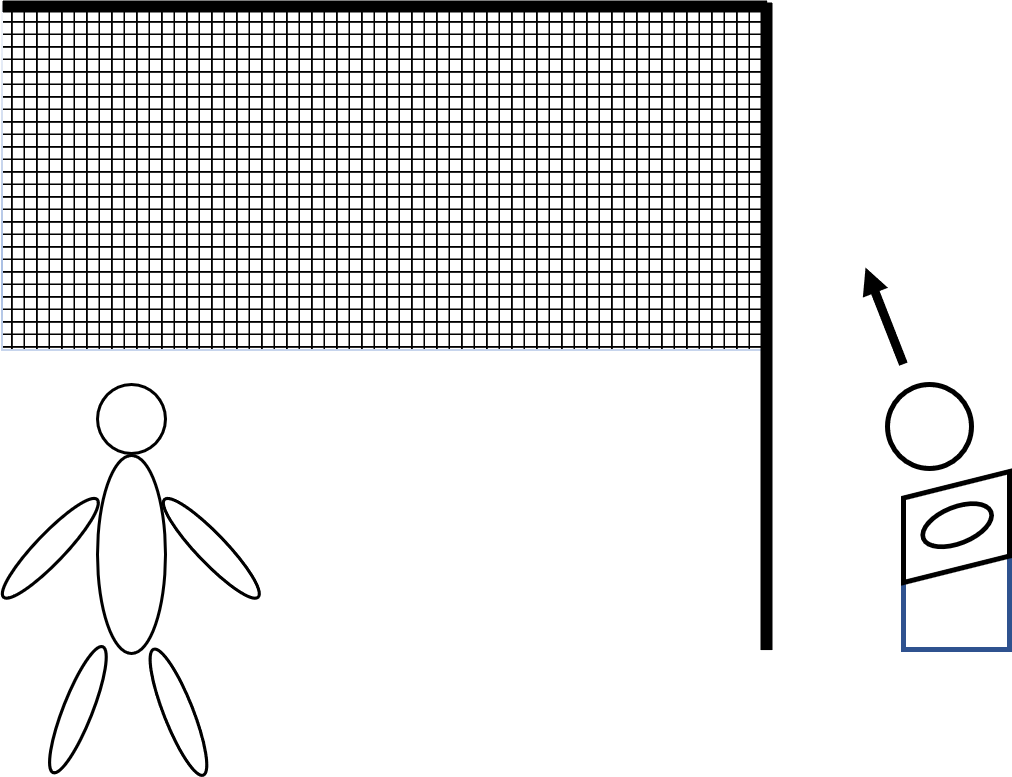
\includegraphics[width = 0.2\textwidth]{spike.png}
  \caption{計測風景}
  \label{}
\end{wrapfigure}
スパイク自体の評価は自己申告とする。10段階ほどで毎回被験者に評価してもらい、それを試技自体の評価とする。

実験プロトコルとしては以下を考えてみた。
\begin{enumerate}
  \item 被験者のジャンプ最高到達点を調べる
  \item 最大跳躍高に対してどれくらいの高さで打つかを決定する
  \item ボールの射出速度ごとに打点への到達時間を求め、その一定時間前に合図を出す\label{loop_Start}
  \begin{itemize}
    \item この一定時間は助走時間より長いことが望ましい。
    \item ボールが放たれてから打点への到達時間が助走時間より短い時は、ボールが射出されるより先に合図がなる。
  \end{itemize}
  \item 被験者は合図を目安に、スパイクを試みる
  \item 慣れたら合図を出すことをやめ、被検者はボールだけを頼りにスパイクを試みる\label{loop_Stop}
  \item \ref{loop_Start}から\ref{loop_Stop}をいろいろな射出速度に対して行う
\end{enumerate}
繰り返しの中で、合図を先に出すのか後に出すのかは検討が必要である。

おそらく、射出速度が大きい時ほど、打点到達点付近の速度も大きくなるので、
タイミングをとるのが難しくなる。
そして予想としては、初心者ほど打点到達点を早く判断し、タイミングが早くなる。
これは実体験に基づいている。
スパイクは高い打点で打った方が有利であると考えやすいため、
初めから高い打点を実現しようとしてしまうと思う。
また、
低い打点→高い打点への適応より、打てない打点→高い打点の適応のほうが
当たらない→当たるの変化が劇的で図りやすいと考える。

逆に射出速度が小さく、助走を早い段階で始めなければいけない状況では、
初心者と上級者でのタイミングの図り方の違いは想像できない。
初心者ほどボールが射出されてからしか反応できないのであろうか。
クイックという技術がバレーにある以上、
セッターがトスをする以前に助走に入る技術は
バレープレーヤーには備わっていそうである。
しかしそれはセッターに上がったレシーブの情報がないと成り立たない技術かもしれなく、
ボールの射出に関しても様々にアレンジできる。

\end{document}